
\section{Operads, props and \texorpdfstring{$E_\infty$}{}-structures} \label{s:operads and props}

In this section we start by reviewing the basic notions of operads and props.
For a more complete presentation we refer the reader to, for example, \cite{markl2008props}.
We then recall from \cite{medina2020prop1} the definition of the finitely presented prop $\M$ having the property that $\UM$ is an $E_{\infty}$-operad.
From the same reference we recall a combinatorial $\UM$-coalgebra structure on simplicial chains and, from \cite{medina2021cubical}, one on cubical chains. 

\subsection{Symmetric (bi)modules}

Let $\S$ be the category whose objects are the natural numbers and whose set of morphisms between $m$ and $n$ is empty if $m \neq n$ and is otherwise the symmetric group $\S_n$.
A \textit{left $\S$ module} (resp. $\S$ \textit{bimodule}) is a functor from $\S$ (resp. $\S \times \S^\op$) to $\Ch$.
We respectively denote by $\smod$ and $\sbimod$ the categories of left $\S$ modules and of $\S$ bimodules with morphisms given by natural transformations.
We notice that the group homomorphisms $\S_n \to \S_n \times \S_1$ induce a forgetful functor $\U \colon \sbimod \to \smod$.

\subsection{Composition structures}

We can define \textit{operads} and \textit{props} by enriching $\S$ modules and \mbox{$\S$ bimodules} with certain composition structures.
For a complete presentation of these concepts we refer to Definition~11 and 54 of \cite{markl2008props}.
Intuitively, using examples defined in the next subsection, operads and props can be understood by abstracting the composition structure naturally present in the left $\S$ module $\End^C$, naturally an operad, and the $\S$ bimodule $\End^C_C$, naturally a prop.

We remark that if $\P$ is a prop, then its composition structure provides $\U(\P)$ with the structure of an operad.

\subsection{Representations}

Given a chain complex $C$ define
\begin{align*}
\End^C(r) &= \Hom(C, C^{\otimes r}), \\
\End^C_C(s, r) &= \Hom(C^{\otimes s}, C^{\otimes r}),
\end{align*}
with their natural operad and prop structures respectively.

Given an operad $\O$, an $\O$-\textit{structure} on $C$ is an operad morphism $\O \to \End^C$.
If equipped with an \mbox{$\O$-\textit{structure}} we say $C$ is an $\O$-coalgebra, denoting the category of these by $\coAlg_\O$.
For a prop $\P$, using $\End_C^C$ we define analogously the notion of $\P$-bialgebra and their category $\biAlg_\P$.

We remark that among these two categories only $\coAlg_\O$ is cocomplete in general.

\subsection{$E_{\infty}$-operads}

An $\S$ module $M$ is said to be $E_{\infty}$-if for each $r$ the chain complex $M(r)$ is an algebraic model for the universal bundle $E\S_r$, i.e., it is free as an $\k[\S_r]$-module and its homology is that of a point.
An operad is said to be $E_{\infty}$-if its underlying $\S$ modules is $E_\infty$.

\subsection{Free constructions} \label{ss:free constructions}

The \textit{free prop} $\F(M)$ generated by an \mbox{$\S$ bimodule} $M$ is constructed using open directed graphs with no directed loops that are enriched with a labeling described next.
We think of each directed edge as built from two compatibly directed half-edges. For each vertex $v$ of a directed graph $G$, we have the sets $in(v)$ and $out(v)$ of half-edges that are respectively incoming to and outgoing from $v$.
Half-edges that do not belong to $in(v)$ or $out(v)$ for any $v$ are divided into the disjoint sets $in(G)$ and $out(G)$ of incoming and outgoing external half-edges. For any positive integer $n$ let $\overline{n} = \{1,\dots,n\}$ and set $\overline{0} = \emptyset$. For any finite set $S$, denote the cardinality of $S$ by $|S|$.
The labeling is given by bijections  
\begin{equation*}
\overline{|in(G)|}\to in(G), \qquad
\overline{|out(G)|}\to out(G),
\end{equation*}
and
\begin{equation*}
\overline{|in(v)|}\to in(v), \qquad
\overline{|out(v)|}\to out(v),
\end{equation*}
for every vertex $v$.
We refer to the isomorphism classes of such labeled directed graphs with no directed loops as $(n,m)$\textit{-graphs} denoting the set of these by $\G(m,n)$.
We use graphs immersed in the plane to represent elements in $\G(m,n)$, please see \cref{f:immersion}.
We consider the right action of $\S_n$ and the left action of $\S_m$ on a $(n,m)$-graph given respectively by permuting the labels of $in(G)$ and $out(G)$.
This action defines the $\S$ bimodule structure on the free prop
\begin{equation} \label{e:free prop}
\F(M)(m,n) \ = \bigoplus_{\Gamma \in \G(m,n)} \bigotimes_{v \in Vert(\Gamma)} out(v) \otimes_{\S_q} M(p, q) \otimes_{\S_p} in(v),
\end{equation}
where we simplified the notation writing $p$ and $q$ for $\overline{|in(v)|}$ and $\overline{|out(v)|}$ respectively.
The composition structure is defined by (relabeled) grafting and disjoint union.

The \textit{free operad} generated by an $\S$-module is defined analogously using $(1,n)$-graphs only.

\begin{figure}
	\begin{tikzpicture}[scale=.6]
\draw (1,3.7) to (1,3); 

\draw (1,3) to [out=205, in=90] (0,0);

\draw [shorten >= 0cm] (.6,2.73) to [out=-100, in=90] (2,0);

\draw [shorten >= .15cm] (1,3) to [out=-25, in=30, distance=1.1cm] (1,1.5);
\draw [shorten <= .1cm] (1,1.5) to [out=210, in=20] (0,1);

\node at (1,3.9){};
\node at (0,-.32){};
\node at (2,-.32){};

\node at (3,1.5){$\sim$\ \ \ };
\end{tikzpicture}
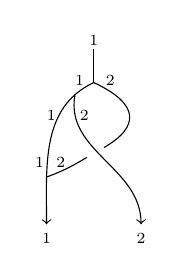
\begin{tikzpicture}[scale=.6]
\draw (1,3.7) to (1,3); 

\draw [->](1,3) to [out=205, in=90] (0,0);

\draw [shorten >= 0cm,->] (.6,2.73) to [out=-100, in=90] (2,0);

\draw [shorten >= .15cm] (1,3) to [out=-25, in=30, distance=1.1cm] (1,1.5);
\draw [shorten <= .1cm] (1,1.5) to [out=210, in=20] (0,1);


\def\x{.8}

\node[scale=\x] at (1,3.9){$\scriptstyle 1$};

\node[scale=\x] at (.7,3.05){$\scriptstyle 1$};
\node[scale=\x] at (1.35,3.05){$\scriptstyle 2$};

\node[scale=\x] at (.1,2.3){$\scriptstyle 1$};
\node[scale=\x] at (.8,2.3){$\scriptstyle 2$};

\node[scale=\x] at (-.15,1.3){$\scriptstyle 1$};
\node[scale=\x] at (.3,1.3){$\scriptstyle 2$};

\node[scale=\x] at (0,-.3){$\scriptstyle 1$};
\node[scale=\x] at (2,-.3){$\scriptstyle 2$};
\end{tikzpicture}
	\caption{Immersed graphs represent labeled directed graphs with the direction implicitly given from top to bottom and the labeling from left to right.}
	\label{f:immersion}
\end{figure}

\subsection{Coalgebras revisited}

We recall the definition operad $\As$ controlling coalgebras in the sense of \cref{ss:coalgebras}.
More precisely, $\As$ is such that there is a natural isomorphisms between $\coAlg_\As$ and $\coAlg$.

\begin{definition}
	Let $\As$ be the operad generated by 
	\begin{equation*}
	\counit\,, \qquad \coproduct\,,
	\end{equation*}
	both in homological degrees $0$ and boundaries
	\begin{equation*}
	\partial\ \counit = 0,
	\hspace*{.6cm}
	\partial\, \coproduct = 0,
	\end{equation*}
	modulo the operad ideal generated by the relations
	\begin{equation*}
	\leftcounitality\,, \hspace*{.6cm} \rightcounitality\,, \hspace*{.5cm} \coassociativity\,.
	\end{equation*}
\end{definition}

We remark that this operad is in any arity $r$ isomorphic to the chain complex $\k[\S_r]$ concentrated in degree~$0$.

\subsection{The prop $\M$} \label{ss:definition of M}

We review from \cite{medina2020prop1} the finitely presented $E_{\infty}$-prop $\M$ which, given its small number of generators and relations, is well suited to define $E_{\infty}$-structures.

\begin{definition}
	Let $\M$ be the prop generated by
	\begin{equation} \label{e:generators of M}
	\counit\,, \hspace*{.6cm} \coproduct\,, \hspace*{.6cm} \product,
	\end{equation}
	in degrees $0$, $0$ and $1$ respectively, and boundaries
	\begin{equation} \label{e:boundary of M}
	\partial\ \counit = 0,
	\hspace*{.6cm}
	\partial\, \coproduct = 0,
	\hspace*{.6cm}
	\partial \product = \ \boundary\,,
	\end{equation}
	modulo the prop ideal generated by
	\begin{equation} \label{e:relations of M}
	\leftcounitality\,, \hspace*{.6cm} \rightcounitality\,, \hspace*{.5cm} \coassociativity\,, \hspace*{.6cm} \productcounit.
	\end{equation}
\end{definition}

Explicitly, any element in $\M(m,n)$ can be written as a linear combination of the $(m,n)$-graphs generated by those in \eqref{e:generators of M} via grafting, disjoint union and relabeling, modulo the prop ideal generated by the relations in \eqref{e:relations of M}, and its boundary is determined, using \eqref{e:free prop}, by \eqref{e:boundary of M}.

Originally this prop was defined without imposing the relation \ \coassociativity \,.
This is advantageous since in that case the associated reduced operad is a cofibrant resolution of the terminal operad.
Since in this work we are interested in extending the Alexander--Whitney and Serre coalgebras, which are coassociative, we find it convenient to impose this relation, so obtaining an inclusion $\As \to \UM$ and a forgetful functor $\coAlg_\UM \to \coAlg$.

The same proof given in \cite[Theorem 3.3]{medina2020prop1} establishes the following.

\begin{proposition}
	The operad $\UM$ is an $E_{\infty}$-operad.
\end{proposition}

\subsection{Simplicial $E_{\infty}$-structure} \label{ss:e-infty on simplicial}

We review from \cite{medina2020prop1} a natural $\mathcal M$-structure on the chains of standard simplices leading to a natural $\UM$-structure on the chains of a simplicial set, generalizing the $E_{\infty}$-coalgebra structures constructed by McClure--Smith \cite{mcclure2003multivariable} and Berger--Fresse \cite{berger2004combinatorial}.

An $\M$-structure is specified by three linear maps, the images of the generators
\begin{equation*}
\counit, \quad \coproduct, \quad \product,
\end{equation*}
satisfying the relations in the presentation of $\mathcal M$.
For the chains on standard simplices, the first two generators are send respectively to the counit and coproduct of the Alexander--Whitney coalgebra as defined in \cref{ss:aw coalgebra}, and the third generator to an algebraic version of the join $\ast \colon \chains(\simplex^n)^{\otimes 2} \to \chains(\simplex^n)$ defined by
\begin{equation*}
\left[v_0, \dots, v_p \right] \ast \left[v_{p+1}, \dots, v_q\right] = \begin{cases} (-1)^{p+|\pi|} \left[ v_{\pi(0)}, \dots, v_{\pi(q)} \right] & \text{ if } v_i \neq v_j \text{ for } i \neq j, \\
0 & \text{ otherwise}, \end{cases}
\end{equation*}
where $\pi$ is the permutation that orders the totally ordered set of vertices, and $(-1)^{|\pi|}$ its sign.

The same proof given in \cite[Theorem 4.2]{medina2020prop1} establishes the following.

\begin{proposition} \label{p:simplicial chain bialgebra}
	For every $n \in \mathbb{N}$, the assignment
	\begin{equation*}
	\counit \mapsto \epsilon, \quad \coproduct \mapsto \Delta, \quad \product \mapsto \ast,
	\end{equation*}
	defines a natural $\mathcal M$-structure on $\chains(\simplex^n)$ extending the Alexander--Whitney coalgebra.
\end{proposition}

The chains on general simplicial sets are not equipped with a $\M$-structure, but using the forgetful functor from $\biAlg_{\M}$ to the cocomplete category $\coAlg_\UM$ allows us to Kan extend the induced natural $\UM$-structures on standard simplices to all simplicial sets.
Specifically, we obtain a lift:
\begin{equation*}
\begin{tikzcd}[column sep=normal, row sep=small]
& \coAlg_\UM \arrow[d] \\
& \coAlg \arrow[d] \\
\sSet \arrow[r, "\schains"]
\arrow[ur, "\schainsAS", out=45, in=180]
\arrow[uur, "\schainsUM", out=90, in=180]
& \Ch.
\end{tikzcd}
\end{equation*}

\subsection{Cubical $E_\infty$-structure} \label{ss:e-infty on cubical}

We follow the presentation of \cref{ss:e-infty on simplicial} closely to review from \cite{medina2021cubical} a natural $\mathcal M$-structure on the chains of standard cubes leading to a natural $\UM$-structure on the chains of any cubical sets.

An $\M$-structure is specified by three linear maps, the images of the generators
\begin{equation*}
\counit, \quad \coproduct, \quad \product,
\end{equation*}
satisfying the relations in the presentation of $\mathcal M$.
For the chains on standard cubes, the first two generators are send respectively to the counit and coproduct of the Serre coalgebra as defined in \cref{ss:serre coalgebra}, and the third generator to a degree one map $\ast \colon \schains(\simplex^n)^{\otimes 2} \to \schains(\simplex^n)$ defined by
\begin{align*}
(x_1 \otimes \cdots \otimes x_n) \ast (y_1 \otimes \cdots \otimes y_n) =
(-1)^{|x|} \sum_{i=1}^n x_{<i} \, \epsilon(y_{<i}) \otimes x_i \ast y_i \otimes \epsilon(x_{>i}) \, y_{>i},
\end{align*}
where
\begin{align*}
x_{<i} & = x_1 \otimes \cdots \otimes x_{i-1}, &
y_{<i} & = y_1 \otimes \cdots \otimes y_{i-1}, \\
x_{>i} & = x_{i+1} \otimes \cdots \otimes x_n, & 
y_{>i} & = y_{i+1} \otimes \cdots \otimes y_n,
\end{align*}
with the convention
\begin{equation*}
x_{<1} = y_{<1} = x_{>n} = y_{>n} = 1 \in \k,
\end{equation*}
and the only non-zero values of $x_i \ast y_i$ are
\begin{equation*}
\ast([0] \otimes [1]) = [0, 1], \qquad  \ast([1] \otimes [0]) = -[0, 1].
\end{equation*}

The same proof given in \cite{medina2020prop1} establishes the following.

\begin{proposition} \label{thm: cubical chain bialgebra}
	For every $n \in \mathbb{N}$, the assignment
	\begin{equation*}
	\counit \mapsto \epsilon, \quad \coproduct \mapsto \Delta, \quad \product \mapsto \ast,
	\end{equation*}
	defines a natural $\mathcal M$-structure on $\chains(\cube^n)$ extending the Serre coalgebra.
\end{proposition}

Kan extending the induced natural $\UM$-structures on standard simplices to all simplicial sets defines a lift of the functor of cubical chains to $\UM$-coalgebras:
\begin{equation} \label{e:lift of cubical chains to UM-coalgs}
\begin{tikzcd}[column sep=normal, row sep=small]
& \coAlg_\UM \arrow[d] \\
& \coAlg \arrow[d] \\
\cSet \arrow[r, "\cchains"]
\arrow[ur, "\cchainsAS", out=45, in=180]
\arrow[uur, "\cchainsUM", out=90, in=180]
& \Ch.
\end{tikzcd}
\end{equation}

In the next section we will show that $\cchainsUM$ is a monoidal functor.